% Od tego momentu porównujemy algorytmy między sobą
\section{Zastosowania}

\subsection{Uwierzytelnianie}
\begin{frame}{Uwierzytelnianie}
    \begin{itemize}
        \pause
        \item Podpisy cyfrowe
        \pause
        \item Certifikaty
    \end{itemize}
\end{frame}

\begin{frame}{Podpisy cyfrowe}
    
\end{frame}

\begin{frame}{Certifikaty}

\end{frame}
\subsection{}
% \subsection{Kryptowaluty}
\begin{frame}{Kryptowaluty}
\begin{center}
    \begin{tabular}{cc}
        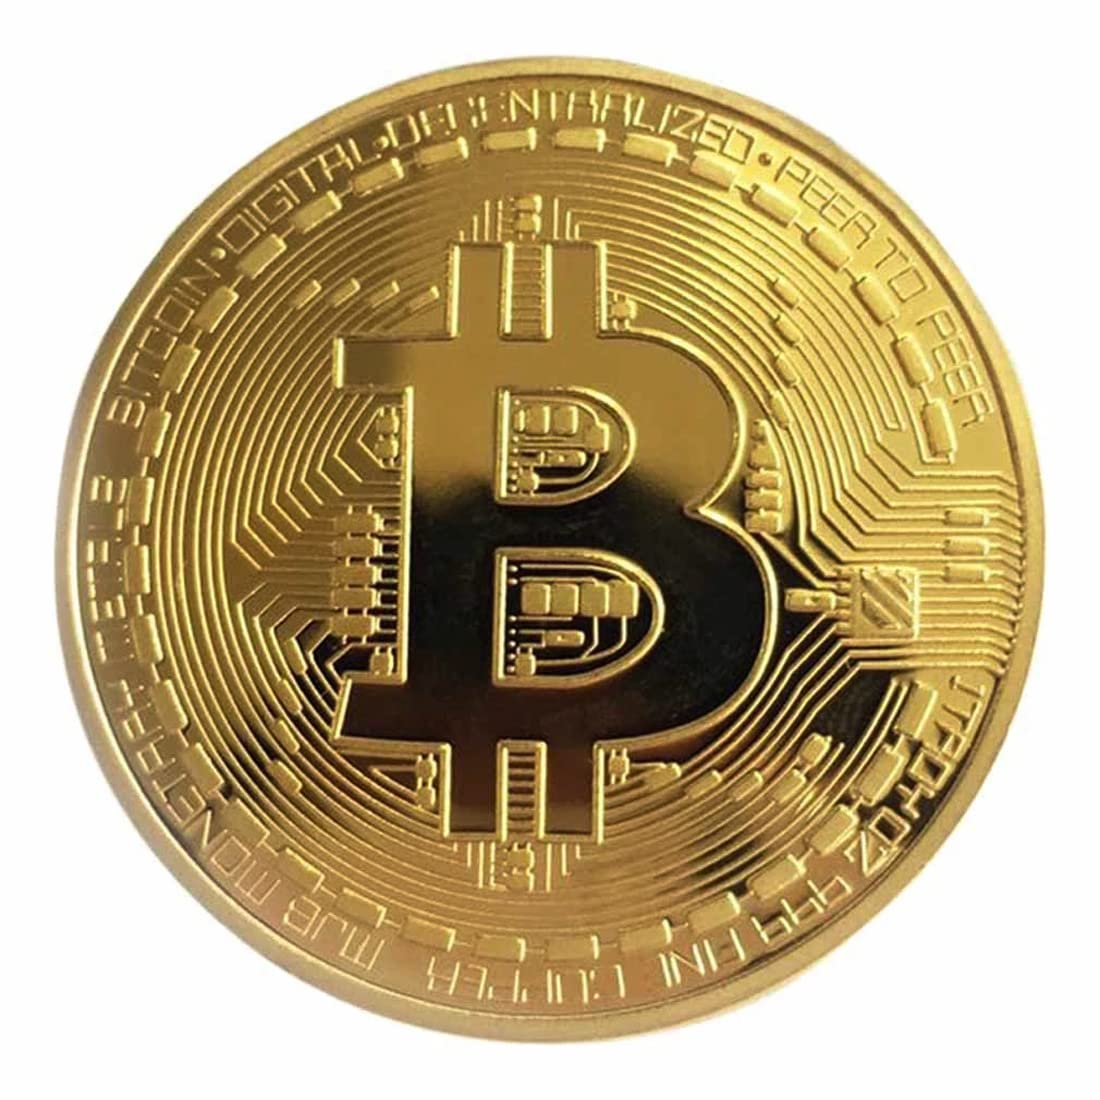
\includegraphics[width=0.3\textwidth, height=0.3\textwidth ]{applications/graphics/Bitcoin.jpg} & 
\includegraphics[width=0.3\textwidth, height=0.3\textwidth]{applications/graphics/Ethereum.png} \\
        
\includegraphics[width=0.3\textwidth, height=0.3\textwidth]{applications/graphics/Dogecoin.png} & 
\includegraphics[width=0.3\textwidth, height=0.3\textwidth]{applications/graphics/Litecoin.jpg} \\
    \end{tabular}
\end{center}
    
\end{frame}

% \subsection{Komunikatory E2E}
\begin{frame}{Komunikatory E2E}
    
\end{frame}

% \subsection{IoT}
\begin{frame}{IoT}
    % Urządzenia mają małą wydajność
    % Szyfrowanie komunikacji HTTP
\end{frame}
